
This chapter shows how encapsulated postscript figures can be included in
the document.  In particular, we wish to show how raw {\tt .eps} and {\tt .pdf}
files can annotated and labeled to make them of ``publication quality''.

\section{A few easy equations and a picture}
\begin{figure}[H]
\setlength{\unitlength}{1mm}
\begin{center}
\setlength{\unitlength}{1mm}
\begin{picture}(100,60)
\dashline{3}(0,45)(100,45)
\dashline{3}(0,42)(100,42)
\drawline(0,5)(100,5)
\put(10,55){\vector(0,-1){50}}
\put(11,50){$\frac{S_{0}}{4}$}
\put(12,5){\vector(0,1){30}}
\put(13,35){$\frac{S_{0}}{4} \alpha_{p}$}
\put(45,5){\vector(0,1){30}}
\put(47,15){$\sigma T^{4}_{s}$}
\put(45,45){\vector(0,1){10}}
\put(47,50){$(1-\epsilon )\sigma T^{4}_{s}$}
\put(80,45){\vector(0,1){10}}
\put(82,47){$\epsilon \sigma T^{4}_{a}$}
\put(80,42){\vector(0,-1){10}}
\put(82,38){$\epsilon \sigma T^{4}_{a}$}
\end{picture} 
 %this works with latex, but not pdflatex
%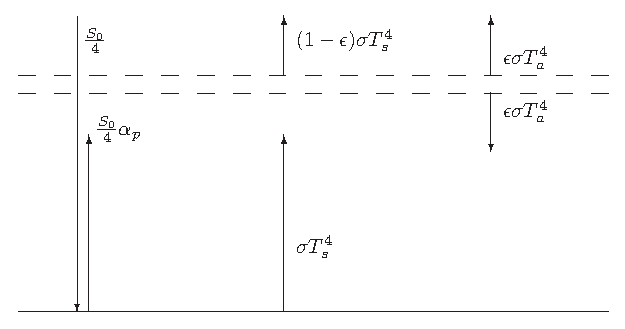
\includegraphics[width=4in]{greenhouse} %uses .pdf in pdflatex, and .eps in latex 
\caption[Radiative equilibrium]{Radiative equilibrium with a ``greenhouse effect''.  This
picture was drawn using \LaTeX\ {\tt epic} commands in the so-called {\em picture
environment}. With {\tt pdflatex}, the horizontal lines will be missing. 
{\tt pdfprob.tar.gz} shows the more complicated procedure to include epic
figures with {\tt pdflatex}.} 
\label{greenhouse}
\end{center}
\end{figure}
A radiative balance at the surface requires that: 
\be
\frac{S_{0}}{4} (1-\alpha_{p})+
\epsilon \sigma T^{4}_{A} 
= \sigma T^{4}_{s}.
\label{surbal}
\ee
Radiative equilibrium of the putative ``atmosphere'' in Figure \ref{greenhouse} requires that:
\be
\epsilon \sigma T^{4}_{s} 
= 2\epsilon \sigma T^{4}_{s}. 
\label{atmosbal}
\ee
We use (\ref{atmosbal}) to eliminate $T_{A}$ from (\ref{surbal}),
which gives:
\be
\frac{S_{0}}{4} (1-\alpha_{p})+
\frac{1}{2}\epsilon \sigma T^{4}_{s} 
= \sigma T^{4}_{s}. 
\label{equi}
\ee
or
\be
T_{s}=\sqrt[4]{
\frac{S_{0}(1-\alpha_{p})}{4\sigma (1-\frac{\epsilon}{2})}}
\ee
\section{Simple inclusion of {\tt .eps} or {\tt .pdf} graphics}
\begin{figure}[H]
\begin{center}
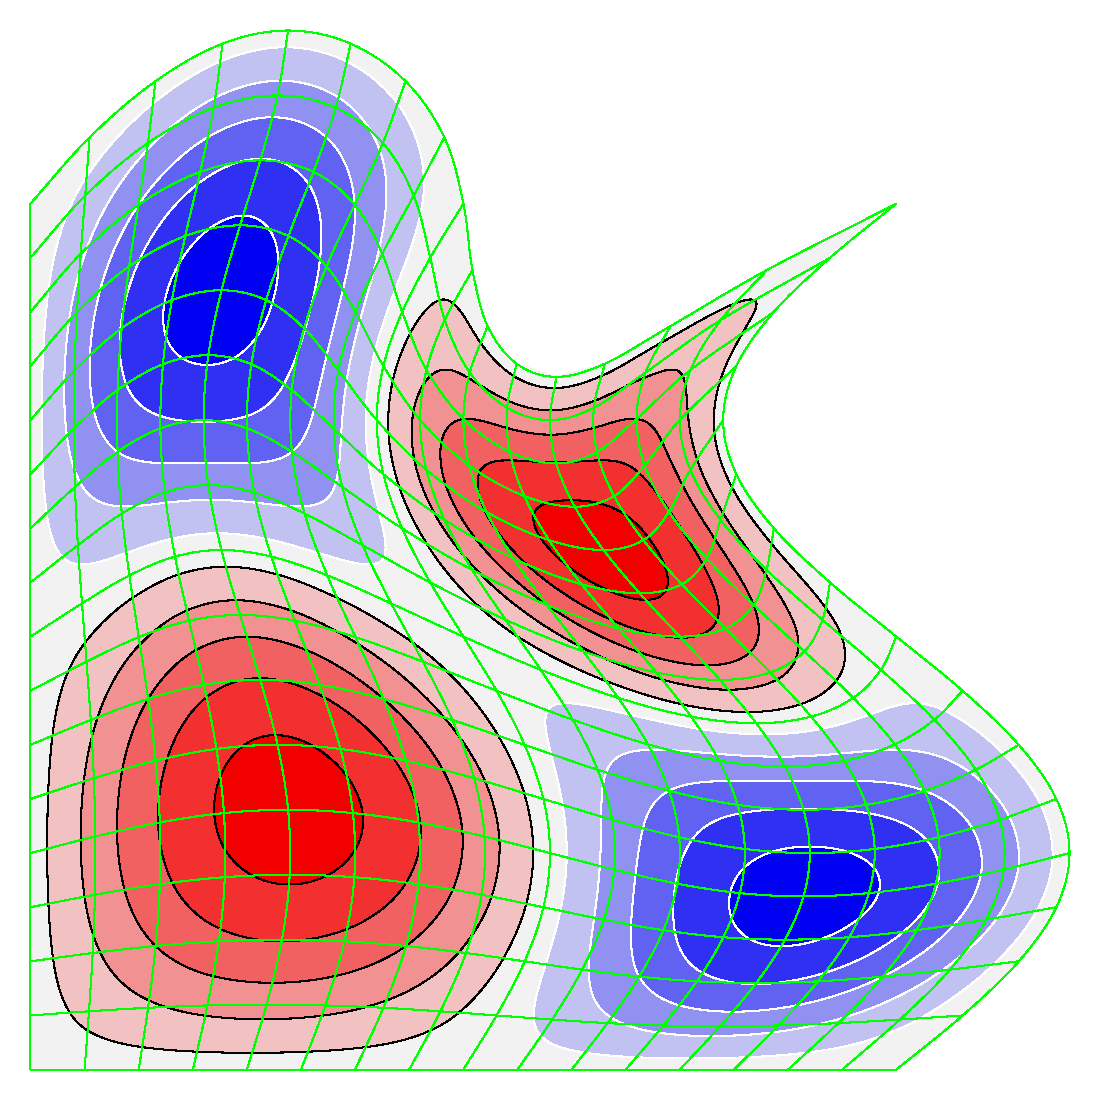
\includegraphics[width=3in]{squash2} 
\end{center}
\caption[Melted figure]{This is what happens when you leave your figure in a hot car
during July.}
\end{figure}
\begin{figure}[H]
\begin{center}
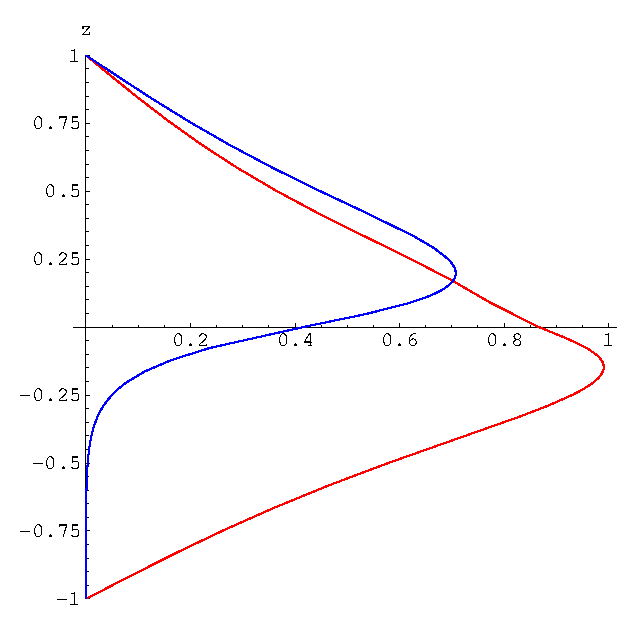
\includegraphics[width=3in]{hitplot}
\end{center}
\caption[Raw {\tt .eps}]{Raw {\tt .eps} from {\bf Mathematica}.}
\end{figure}
%%%%
\section{{\tt .eps or .pdf}, annotated }
\begin{figure}[H]
\setlength{\unitlength}{1in}
\begin{center}
\begin{picture}(3,3)(0,0)
\put(.2,.2){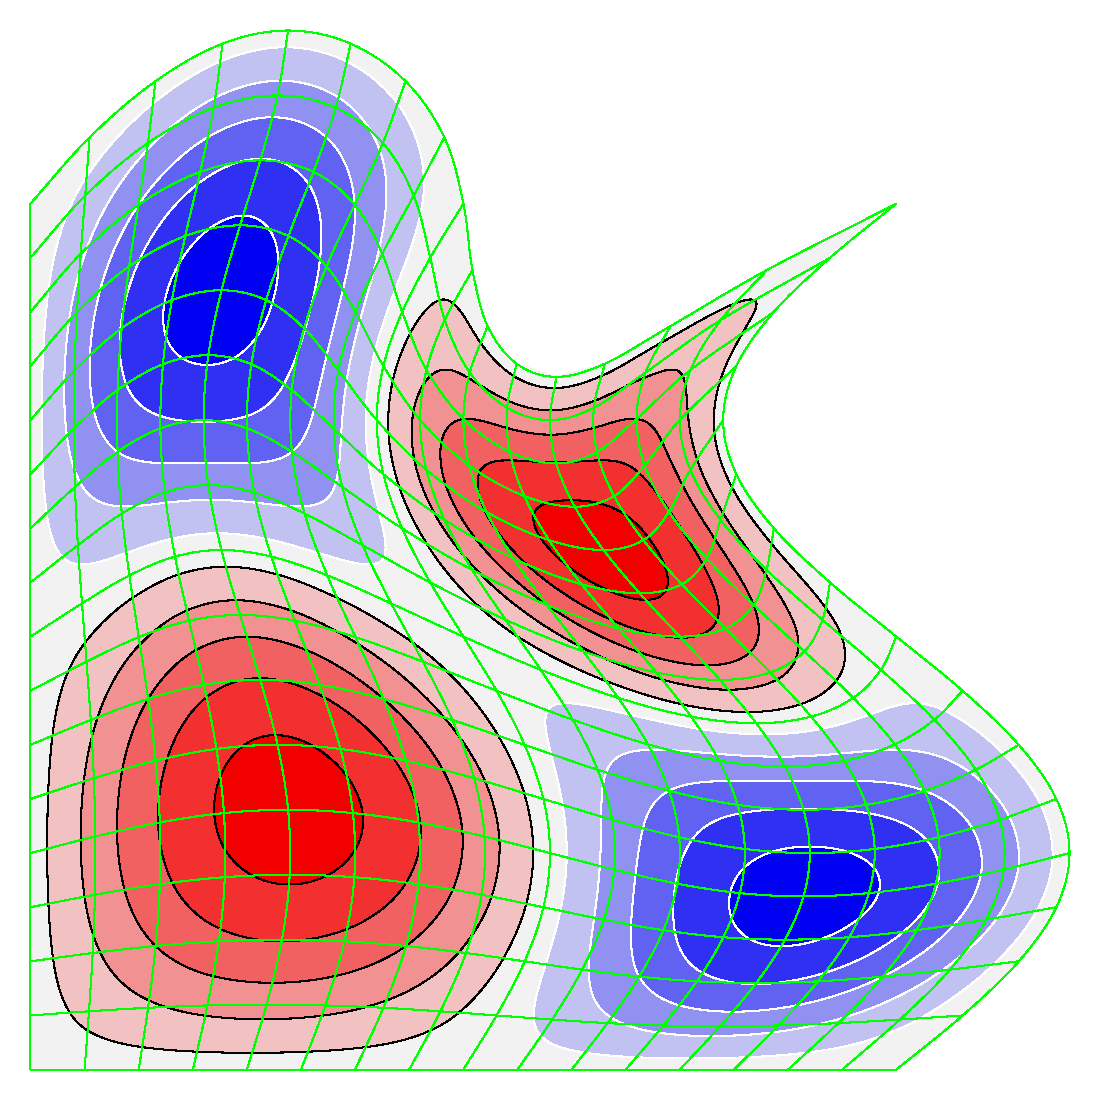
\includegraphics[width=2.6in]{squash2}}
\put(1.7,.1){\vector( 1,0){1.1}}
\put(1.3,.1){\vector(-1,0){1.1}}
\put(1.5,.1){\makebox(0,0)[c]{$\int x dx$}}
\put(.1,1.7){\vector( 0,1){1.1}}
\put(.1,1.3){\vector(0,-1){1.1}}
\put(.1,1.5){\makebox(0,0)[c]{$\frac{y}{x}$}}
\put(1.4,2.2){$E=mc^2$}
\end{picture}
\end{center}
\caption[Annotated melted figure]{The melted figure with annotations.
Wonderful! All of the epic commands here work in both {\tt latex} and {\tt pdflatex},
in Fig. \ref{greenhouse} some did 
did not in {\tt latex}.  This is may favorite way to put labels on my figures.}
\end{figure}
%%%%%%%%%
\section{Using the {\tt psfrag} system with .eps}
\begin{figure}[H]
\begin{center}
\psfrag{z}{\Large $\zeta$}
\setlength{\unitlength}{1in}
\begin{picture}(2.5,2.5)(0,0)
\put(0,0){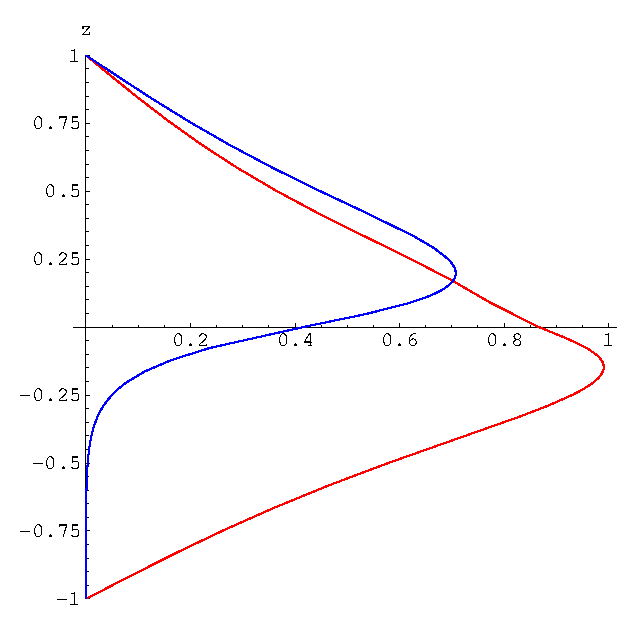
\includegraphics[height=2.5in]{hitplot}}
\put(1.6,.45){$\widehat{\psi}_{r}$}
\put(.5,.8){$\widehat{\psi}_{i}$}
\end{picture}
\end{center}
\caption[Use of {\tt psfrag} system]{This looks ugly until rendered in postscript.
 At that time, the
{\tt z} (which has now vanished) is turned into a $\zeta$.  This will not work
with {\tt pdflatex}.} 
\end{figure}
%%%%%%%%%%%%
